\documentclass[11pt]{article}


\usepackage[sort]{natbib}
\usepackage{bm,amsmath,bbm,amsfonts,nicefrac,latexsym,amsmath,amsfonts,amsbsy,amscd,amsxtra,amsgen,amsopn,bbm,amsthm,amssymb,graphicx}
\usepackage{wrapfig, caption, subcaption}
\usepackage{fancyhdr}
\usepackage[margin=1.0in]{geometry}
\bibliographystyle{plainnat}



\title{Fourth Monitoring Committee Meeting\\\vspace{4mm} \normalsize{Understanding the Information Content in Diverse Observations of Forest Carbon Stocks and Fluxes for Data Assimilation and Ecological Modeling\\ NERC case partnership with Forest Research}}
\author{\normalsize{E. Pinnington}}


\newtheorem{theorem}{Theorem}[section]
\newtheorem*{defn}{Definition}



	
\begin{document}

\maketitle

\section{Introduction}

Forest ecosystems play a large role in reducing the impact of anthropogenic CO$_2$ emissions and therefore understanding their response to climate change is important. Currently, in data assimilation, the optimal set of observations to add the most information to models of forest carbon balance is not known.  

In our last monitoring committee we saw some results of information content experiments using the Data Assimilation Linked Ecosystem Carbon model (DALEC) \citep{williams2005improved} taken from a report I had written. The report had focused mainly on Shannon Information Content (SIC) \citep{rodgers2000inverse} and Degrees of Freedom for Signal (DFS) \citep{fowler2011measures} as measures for information content in carbon balance observations. It was shown previously that a single observation of the Net Ecosystem Exchange (NEE) of CO$_2$ taken in summer with warmer temperatures and higher daily irradiances had a higher information content than those taken in winter. This made physical sense as observations of NEE in the summer are of greater magnitude and give more information about the fluxes of carbon throughout the forest. In the report on information content this was explored further and it was shown that it would take 30 days of successive NEE observations in winter to give the same amount of information as a single NEE observation made in summer.

In the last report DALEC was also implemented in a Four-Dimensional Variational assimilation (4D-Var) scheme for state estimation, where our state corresponded to the 5 initial carbon pool values in DALEC. We used this scheme to assimilate observations of NEE with DALEC using data from an evergreen forest in Oregon. It was shown that assimilating NEE observations not only improved our models estimate of NEE but also improved modelled Gross Primary Production (GPP) and Total ecosystem Respiration (RT). The field work I had been doing at the Alice Holt forest with my case partner Forest Research was also outlined in the last report.

Since completing the last report a new version of the DALEC model was released (DALECV2 \citep{Bloom2014}) and I have built this into a 4D-Var scheme for parameter and state estimation. It was decided to begin work on DALECV2 as it can be parameterised for both deciduous and evergreen forests and the Alice Holt research site is a mainly deciduous forest. Whereas the version of DALEC previously used was a model of  evergreen forests only. We are currently using data acquired from Alice Holt to run DALECV2 and I have worked on getting the driving data and NEE observations into the right format for use with DALECV2.

I have also now completed taking a set of stem respiration observations for Forest Research at the Alice Holt flux site and am now in the early stages of planning a campaign to take leaf area index measurements at the Alice Holt flux site. I have completed a PhD plan which is included along with the monitoring report.            

\section{DALECV2}

The DALECV2 model is a simple process-based model describing the carbon balance of a forest ecosystem \citep{Bloom2014} and is the new version of the original DALEC \citep{williams2005improved}. The model is constructed of six carbon pools (labile ($C_{lab}$), foliage ($C_f$), fine roots ($C_r$), woody stems and coarse roots ($C_w$), fresh leaf and fine root litter ($C_l$) and soil organic matter and coarse woody debris ($C_s$)) linked via fluxes. The aggregated canopy model (ACM) \citep{williams1997predicting} is used to calculate daily gross primary production ($GPP$) of the forest, taking meteorological driving data and the site's leaf area index (a function of $C_f$) as arguments.   

\begin{figure}[ht]
    \centering
    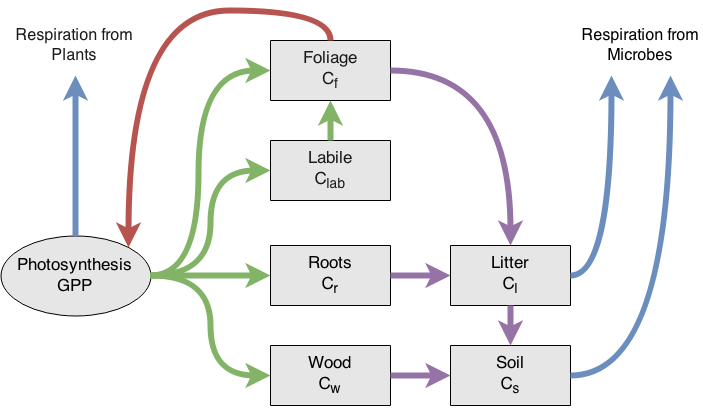
\includegraphics[width=0.5\textwidth]{Dalecdiagram.png}
    \caption{Representation of the fluxes in the DALEC2 carbon balance model. Green arrows represent C allocation, purple arrows represent litter fall and decomposition fluxes, blue arrows represent respiration fluxes and the red arrow represents the feedback of foliar carbon to the $GPP$ function.}
    \label{fig:DALEC_mod}
\end{figure}

\section{4D-Var}

In 4D-Var we aim to maximise the probability of our initial state $\textbf{x}_0$ given a set of observations $\textbf{y}$, $P(\textbf{x}_0|\textbf{y})$, over some time window, $N$. $P(\textbf{x}_0|\textbf{y})$ is maximised by minimising a cost function $J(\textbf{x})$ derived from Baye's Theorem \citep{lewis2006dynamic}. The cost function is given as,

\begin{equation}
J(\textbf{x}_0) = \frac{1}{2}(\textbf{x}_0-\textbf{x}_b)^{T}\textbf{B}^{-1}(\textbf{x}_0-\textbf{x}_b)+\frac{1}{2}\sum_{i=0}^{N}(\textbf{y}_i-h_i(\textbf{x}_i))^{T}\textbf{R}_{i}^{-1}(\textbf{y}_i-h_i(\textbf{x}_i)),
\end{equation}

where $\textbf{x}_b$ is our background and acts as our initial guess to our state $\textbf{x}_0$, $\textbf{B}$ is the background error covariance matrix and quantifies our knowledge of the error in our background, $h_i$ is our observation operator at time $t_i$ and maps our state vector evolved by our nonlinear model ($m_{0\rightarrow i}(\mathbf{x}_{0})=\textbf{x}_i$) to the observations at this time ($\textbf{y}_i$) and $\textbf{R}_i$ is the observation error covariance matrix at time $t_i$ and represents our knowledge of the uncertainty in the observations. The state that minimises the cost function is called the analysis and is denoted as $\textbf{x}_a$, this state is found using a minimisation routine that takes the cost function, our initial guess ($\textbf{x}_b$) and also the gradient of the cost function defined as,

\begin{equation}
\nabla J(\textbf{x}_0) = \textbf{B}^{-1}(\textbf{x}_0-\textbf{x}_b)-\sum_{i=0}^{N}\textbf{M}_{i,0}^{T}\textbf{H}_i^{T}\textbf{R}_{i}^{-1}(\textbf{y}_i-h_i(\textbf{x}_i)),
\end{equation}

where $\textbf{H}_i = \frac{\delta h_i(\textbf{x}_i)}{\delta\textbf{x}_i}$ is our linearized observation operator and $\mathbf{M}_{i,0}=\mathbf{M}_{i-1}\mathbf{M}_{i-2}\cdots\mathbf{M}_0$ is our tangent linear model with $\mathbf{M}_i=\frac{\delta m_{i}(\textbf{x}_{i})}{\delta \textbf{x}_{i}}$. We can rewrite the cost function and its gradient to avoid the sum notation as,

\begin{equation}
J(\textbf{x}_0) = \frac{1}{2}(\textbf{x}_0-\textbf{x}_b)^{T}\textbf{B}^{-1}(\textbf{x}_0-\textbf{x}_b)+\frac{1}{2}(\hat{\textbf{y}}-\hat{h}(\textbf{x}_0))^{T}\hat{\textbf{R}}^{-1}(\hat{\textbf{y}}-\hat{h}(\textbf{x}_0)) \label{costfn}
\end{equation}
and
\begin{equation}
\nabla J(\textbf{x}_0) = \textbf{B}^{-1}(\textbf{x}_0-\textbf{x}_b)-\hat{\mathbf{H}}^{T}\hat{\textbf{R}}^{-1}(\hat{\textbf{y}}-\hat{h}(\textbf{x}_0)), \label{gradcostfn}
\end{equation}
where,
\begin{equation}
\hat{\textbf{y}}=
\begin{pmatrix}
\textbf{y}_0 \\
\textbf{y}_1\\
\vdots \\
\textbf{y}_N
\end{pmatrix},
\hspace{1mm}
\hat{h}(\textbf{x}_0)=
\begin{pmatrix}
h_0(\textbf{x}_0) \\
h_1(m_{0\rightarrow 1}(\mathbf{x}_{0}))\\
\vdots \\
h_N(m_{0\rightarrow N}(\mathbf{x}_{0}))
\end{pmatrix},
\hspace{1mm}
\hat{\mathbf{R}}=
\begin{pmatrix}
\mathbf{R}_0 & 0 & 0 & 0 \\
0 & \mathbf{R}_1 & 0 & 0 \\
0 & 0 & \ddots & 0 \\
0 & 0 & 0 & \mathbf{R}_N
\end{pmatrix}
\hspace{1mm} \text{and} \hspace{3mm}
\hat{\mathbf{H}}=
\begin{pmatrix}
\mathbf{H}_0 \\
\mathbf{H}_1\mathbf{M}_0\\
\vdots \\
\mathbf{H}_N\mathbf{M}_{N,0}
\end{pmatrix}.
\end{equation}

\section{4D-Var with DALECV2}

In our DALECV2 4D-Var scheme the state vector, $\textbf{x}_0$, corresponds to the vector of the 17 model parameters and 6 initial carbon pool values. We use a diagonal approximation to our background and observational error covariance matrices so that, 
$\textbf{B}=\underline{\sigma}_b^2 \textbf{I}$ and $\hat{\textbf{R}}=\underline{\sigma}_o^2 \textbf{I}$,
where $\underline{\sigma}_b$ and $\underline{\sigma}_o$ are the vectors of the background and observational standard deviations respectively.

In order to find the tangent linear model (TLM) for DALECV2 we need to find the derivative of the model at each time step with respect to the 17 model parameters and the 6 carbon pools. Previously the DALEC TLM was calculated by hand, however, now that we are working with a more complex model and an extra 18 state members we use the AlgoPy automatic differentiation package in Python. It is important to test the tangent linear hypothesis as we did with the original DALEC. In 4D-Var we assume the tangent linear hypothesis,
\begin{equation}
m_{0\rightarrow i}(\mathbf{x}_0+\delta\mathbf{x}_0) \approx m_{0 \rightarrow i}(\mathbf{x}_0) + \mathbf{M}_{i,0}\delta\mathbf{x}_0. \label{TLH}
\end{equation}
The validity of this assumption depends on how nonlinear the model is, the length of the assimilation window and the size of the perturbation $\delta\mathbf{x}_0$. We can test the validity for DALECV2 by taking an initial state $\mathbf{x}_0$ and a $5\%$ perturbation for $\delta\mathbf{x}_0$. We then rearrange equation \ref{TLH} to find, 
\begin{equation}
\text{percentage error in TLM} = \begin{vmatrix} \frac{m_{0\rightarrow i}(\mathbf{x}_0+\delta\mathbf{x}_0) - m_{0 \rightarrow i}(\mathbf{x}_0)}{ \mathbf{M}_{i,0}\delta\mathbf{x}_0} - 1 \end{vmatrix} \times 100.
\end{equation}

\begin{figure}[ht]
    \centering
    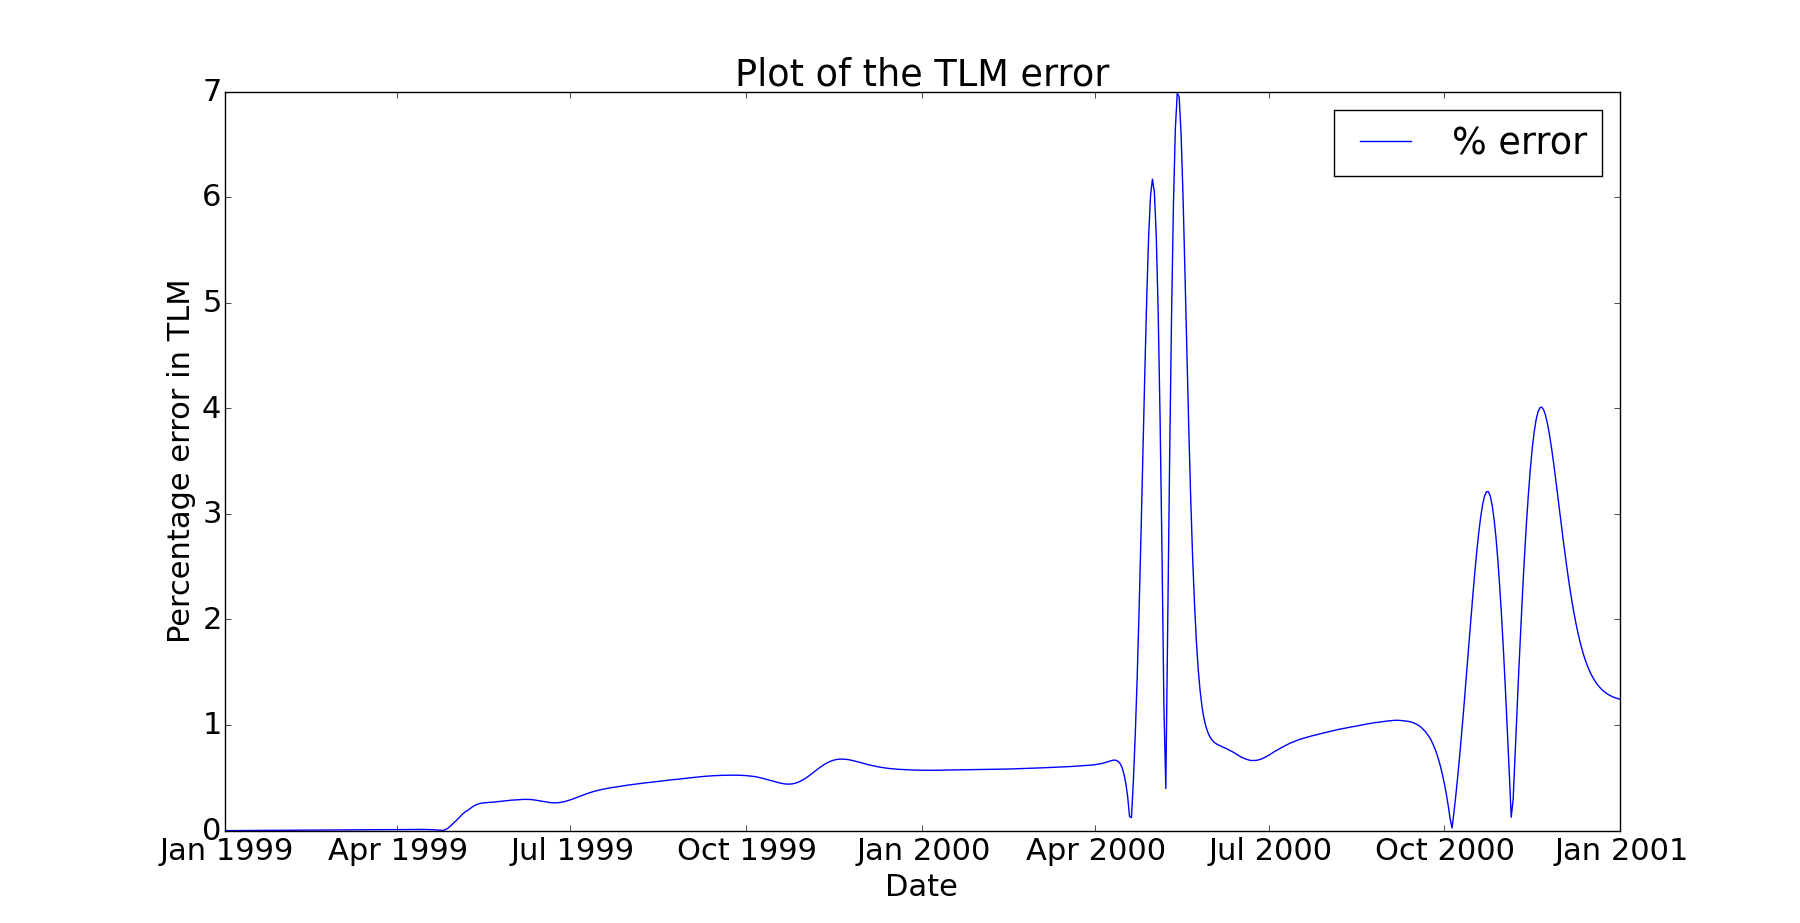
\includegraphics[width=0.8\textwidth]{tlm_error.png}
    \caption{Plot of the percentage error in our tangent linear model for DALECV2 when evolving our state forward over a period of two years.}
    \label{fig:tlm_error}
\end{figure}

In figure \ref{fig:tlm_error} we can see that our TLM for DALECV2 performs very well after being run forward a year with less than a $1\%$ error. By the second year we see some peaks in our error in spring and autumn, this is where functions controlling leaf on and leaf off in the nonlinear DALECV2 have gone out of phase with the TLM. Even at these peaks our error is still reasonable reaching a maximum at $7\%$ and then coming back to around $1\%$. 

In figure~\ref{fig:4dvar} we see a 4D-Var run using NEE observations and meteorological driving data from Alice Holt. Here we are using a truncated Newton method \citep{Nocedal1999} from the Python package Scipy.optimize to find the minimum of our 4D-Var cost function. Our $\textbf{x}_b$ is a parameter set found by the University of Edinburgh using the CARbon DAta-MOdel fraMework (CARDAMOM) \citep{Exbrayat2015}. This used Harmonised World Soil Database $C_{s}$ observations as initial conditions, meteorological driving data from ERA-interim and Markov chain Monte Carlo techniques to assimilate MODIS leaf area index observations over a 10 year period. 

\begin{figure}[!hb]
    \centering
    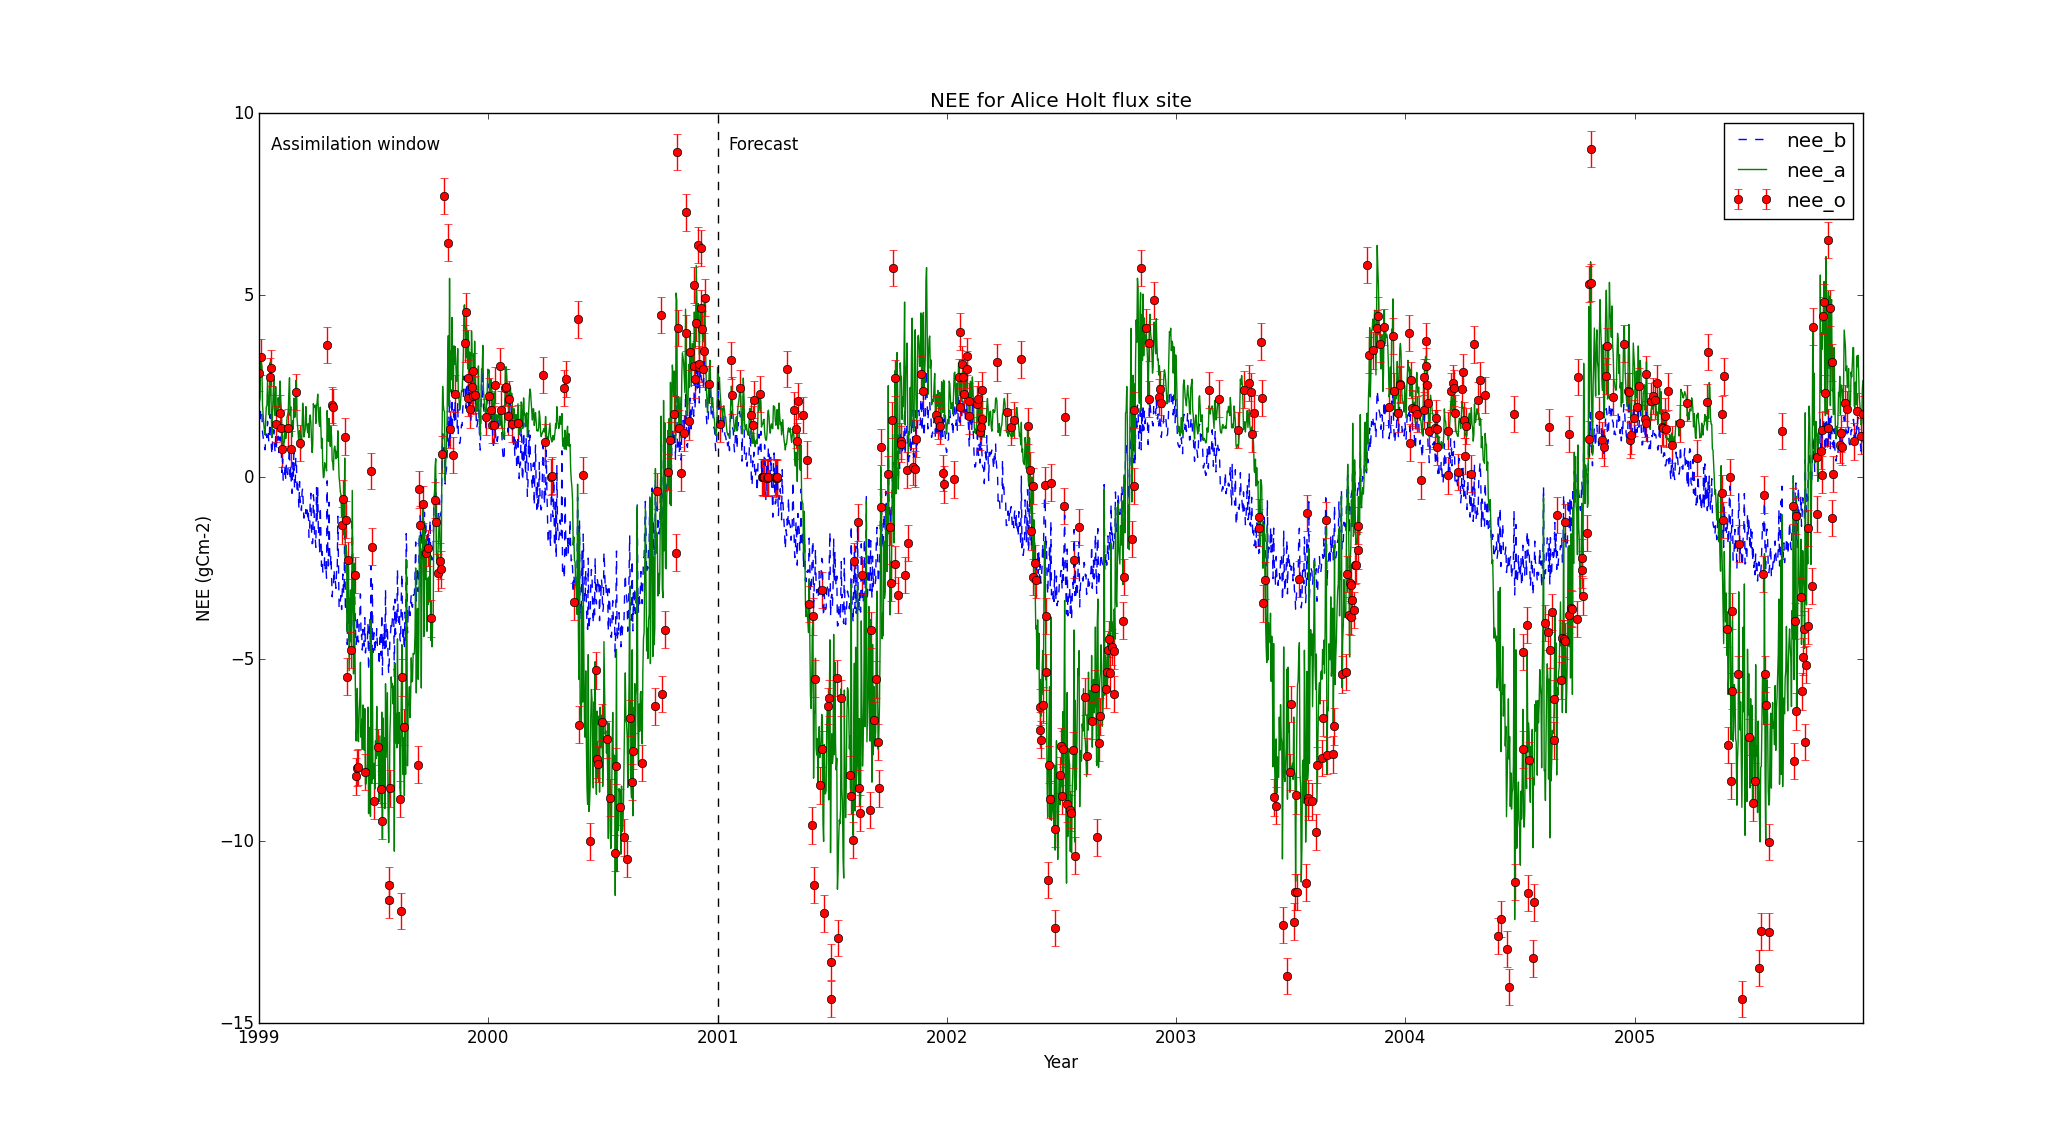
\includegraphics[width=.9\textwidth]{ah_assim_edinpvals.png}
    \caption{4D-Var run for Alice Holt flux site, assimilating NEE observations from 1999-2001. The red dots are our observations, the blue dotted line our background estimate and the green line is our analysis.}
    \label{fig:4dvar}
\end{figure}

From figure~\ref{fig:4dvar} we can see that after assimilating NEE observations from 1999-2001 and then running our analysis forward from 2001-2006 we have a much better forecast of NEE than we did from our initial background guess (when judging against observations). 

I am currently working on getting DALECV2 coded up with a 4D-Var scheme in Python, with a state made up of the initial carbon pool values and the 17 model parameters so that the model can be parameterised for the Alice Holt research site.


\section{Current Work and Future Plans}

I am currently repeating the information content experiments conducted with DALECV2. While applying the measures previously used (SIC and DFS) I am also starting to work with the influence matrix \citep{Cardinali2004} and the adjoint technique proposed by \cite{Langland2004}. The influence matrix is defined as,
\begin{equation}
\textbf{S} = \frac{\delta \hat{\mathbf{H}}\textbf{x}_a}{\delta \hat{\textbf{y}}} = \hat{\textbf{R}}^{-1}\hat{\mathbf{H}}\textbf{A}\hat{\mathbf{H}}^{T},
\end{equation}

where $\textbf{A}$ is our analysis error covariance matrix. Using these measures and an observing system simulation experiment I have developed I will produce another report investigating the best set of observations for understanding the carbon balance of a forest and apply the results to the available data from Alice Holt. 

I am also in the very early stages of planning a fieldwork campaign at Alice Holt. In this campaign I will be taking measurements of leaf area index using a ceptometer and hemispherical photographs. Tristan and I have meeting with Forest Research on the $28^{th}$ May to further plan the fieldwork. These measurements will be used in the information content experiments but also to address site specific science questions. Half of the Alice Holt forest has been thinned and the other half left unmanaged.  The flux tower measuring NEE is placed directly on the boundary of the two halves. The leaf area index measurements will allow us to compare the difference between the two sides and also evaluate DALECV2's estimate of leaf area index. We will also parameterise two versions of DALECV2 for the thinned/unthinned forest using NEE observations and a tower foot print model to split the NEE observations when the signal is coming from the thinned or unthinned side of the forest. We will then be able to see if by just assimilating NEE we can pick out a difference in LAI between the two sides.

Other future work will be based on the attached PhD outline. This includes attempting to improve the representation of background and observational error covariance matrices in DALECV2. This is important as improving our representation of these matrices could lead to different results in the information content experiments.  



\section{Professional and Academic Development}

\subsection{Masters Courses}
\begin{itemize}
\item MAMB10 (Data Assimilation) - 85\%
\item MAMNSO (Numerical Solutions to Ordinary Differential Equations) - 79\%
\item MTMG02 (Atmospheric Physics) - 66\%
\item MTMG49 (Boundary Layer) - 72\%
\item MTMD01 (Environmental Data Visualization) - 78\%
\item MTMD02 (Operational Data Assimilation) - 70\%
\end{itemize}

\subsection{Transferable Skills}

During my PhD I have taken part in the following courses, workshops and activities:
\begin{itemize}
\item 28/01/2014 - Basic Statistics Refresher - RRDP

\item 31/03/2014-01/04/2014 - Land Data Assimilation workshop at UCL - ESA

\item 23/04/2014-25/03/2014 - Correlated Observation Errors in Data Assimilation Workshop - ESA

\item 13/05/2014 - Social Media - Bloggs, Twitter and Your Online Presence - RRDP

\item 29/05/2014 - How to Write a Paper - RRDP

\item 25/06/2014-26/06/2014 - Software Carpentry Course - Git and Python

\item 10/07/2014-11/07/2014 - Forest Research - Helped with field work LiDAR

\item  21/07/2014-01/08/2014 - Fluxcourse Summer School - University of Colorado

\item 29/09/2014-03/10/2014 - NERC course - Software Development for Environmental Scientists Level 1

\item 08/10/2014-10/10/2014 - Environment YES - NERC ``dragon's den" type competition at Syngenta, Jesops Hill

\item 17/12/2014 - Presentation at Maths for Planet Earth Industry day

\item 24/02/2015 - Reading Soil Centre Workshop - What can Land Surface Models do for you?

\item 23/03/2015-27-03/2015 - NERC course - Software Development for Environmental Scientists Level 2
\end{itemize}

\subsection{Demonstrating}
During my PhD I have helped demonstrate on the following courses:
\begin{itemize}
\item 15/09/2014-1909/2014 - NERC Data assimilation for environmental scientists training course

\item 16/02/2015-20/02/2015 - NERC Software Development for Environmental Scientists Level 1

\item 20/04/2015-23/04/2015 - MT26E Surface Energy Exchange Practicals
\end{itemize}


\bibliography{../../PhD}{}
%\bibliographystyle{plain}
\end{document}